\documentclass[TheoreticalPhy_ModB.tex]{subfiles}
\begin{document}

\chapter{Weak Interactions}

\textsf{Mandl sec. 16.1; Halzen sec. 12.Introduction; \footnote{Beside bibliography, for this chapter some good references can be found in the following sites:\\\url{https://www.imsc.res.in/~graj/genGRaja.pdf}\\\url{http://polywww.in2p3.fr/~paganini/ch6.pdf}\\These reference are used in the following sections even if not cited.}}\\

The Weak interactions theory was born after, in the study of $\beta$-deday\footnote{The theory of $\beta$-decay was developed by W. Pauli in 1934. To solve the puzzle of the continuous energy spectrum of the electrons emitted in the beta decay of nuclei, Pauli had suggested that along with the electron, an almost massless neutral particle also was emitted. This particle was named by Fermi as \emph{neutrino}.}, scientist discovered a process that couldn't be described by QED, namely the neutron decay:
\[n\to p+e^-+\bar \nu_e\]
where $n$ is the neutron, $p$ is the proton, $e^-$ is the electron and $\bar\nu_e$ is the antineutrino. 
From the energy spectrum of out-coming $e^-$ particles scientist understood that this is a 3 body decay. Notice also that netrunos ($\nu_e$ and $\bar \nu_e$) are fermions that couldn't be discovered by detectors since they have no charge. This is the sketch of this interaction:\footnote{We used different colors for different charge currents and different line thickness to distinguish nucleons by smaller fermions.}
\[
\begin{tikzpicture}[baseline=(e0)]
\begin{feynman}[large]
\vertex[blob](e0){\hspace{1cm}};
\vertex[left=of e0](n){$n$};
\vertex[above right=of e0](p){$p$};
\vertex[right=of e0](e){$e^-$};
\vertex[below right=of e0](nu){$\bar\nu_e$};
\diagram*{
	(n) --[fermion, ultra thick](e0),
	(e0) --[fermion, ultra thick, red](p),
	(e0)--[fermion, blue](e),
	(nu)--[fermion](e0),
};
\end{feynman}
\end{tikzpicture}
\]

This new interaction can't be described using QED and two photons that mediate the interactions because of the charge and the spin conservation. 

Before proceeding, we note that it is conventional to divide weak interaction processes into three categories, depending on whether leptons and/or hadrons are involved. Accordingly, we distinguish:
\begin{enumerate}
\item \emph{purely leptonic} processes like
\[\mu^-\to\, e^-\bar\nu_e\nu_\mu\]
which involve only the charged leptons $e^pm$, $\mu^\pm$, $\tau^\pm$ and their associated neutrinos $\nu_e$, $\nu_\mu$, $\nu_\tau$ and antineutrinos $\bar\nu_e$, $\bar\nu_\mu$, $\bar\nu_\tau$
\item \emph{semileptonic} processes involving both hadrons and lepton, like neutron $\beta$-decay
\[n\to\, pe^-\bar\nu_e\]
and 
\[\pi^\mp\to\,\mu^\mp\overset{(-)}{\nu}_\mu\]
\item \emph{purely hadronic} processes like the $\Lambda$ decay
\[\Lambda\to\, p\pi^-\]
and
\[K^+\to\,\pi^+\pi^0\]
\end{enumerate}

Unfortunately we have only a limited understanding of hadrons structure, since the strong forces which bind the wearks act over distances of order 1 fm, where they cannot be treated in perturbation theory. In contrast, we belive that perturbation theory is valid for weak and electromagnetic interactions, and that we understand the latter. Consequently purely leptonic processes afford an unambiguous and far simpler field for studying weak interactions, and we shall restric ourselves to purely leptonic processes. This is analogous to our treatment of QED, where we also did not consider hadrons. 

\section{Four Fermions Fermi Theory and $V-A$ Theory}\label{sec:4-fermions-and-VA}
\textsf{Halzen sec. 12.1; Maggiore sec. 8.1}\\

In 1934 Fermi proposed his theory to describe $\beta$-decay process $n\to p+e^-+\bar \nu_e$. In QED the electromagnetic current $q(\bar e\gamma^\mu e)$ of the charged particle like the electron interacts with the electromagnetic vector potential $A_\mu$, which becomes the field operator for the photon:
\[\mathcal L=q(\bar e\gamma^\mu e)A_\mu\]
The electric current and the vector potential are vectors and so Fermi adopted the vector form for the weak currrents also. 
In Fermi's theory of weak interactions, the weak current of the proton-neutron pair interacts with the weak current of the electron-neutrino pair:
\[\mathcal L_{\text{F}}=\frac{G_F}{\sqrt 2}\p{\bar p\gamma^\mu n}\p{\bar e \gamma_\mu\nu_e}\]
where the particle symbols represent the corresponding field operators. The strength of the weak interaction is characterized by the constant $G_F$ called \textbf{Fermi constant}. The value of $G_F$ is very small, and therefore this interaction is called ``weak''. This lagrangian describes 4 fermions interaction, and therefore is called \textbf{Four Fermions Fermi Lagrangian}. A new coupling constant meant a new force was born. Moreover, the currents in the latter Lagrangian are charged while in QED they are always neutral. Perturbation theory based on this Lagrangian described pretty well the $\beta$-decay.

Since lagrangian has to be 4-dimensional and all these fields have dimension $3/2$ the Fermi constant must have dimension
\[[G_F]=4-6=-2\]
i.e. this theory is not renormalizable since $D=2+2V-E_B-3E_F/2>0$. We will use the SM to obtain a renormalizable theory of weak interactions. 

\subsection{Modification of Fermi's theory: the $V$ - $A$ current}
\textsf{Mandl sec. 16.2, Maggiore sec. 8.2}\\

This theory of weak interactions proposed by Fermi almost 80 years ago purely on an intuitive basis stood the test of time inspite of many amendments that were incorporated into Fermi's theory successfully.  One important amendment came after in 1957 Wu found a Parity violation ($\slashed P$) in Weak interaction, since the $e^-$ produced in the neutron decay is mostly left handed. Fermi's theory survived even this fundamental revolution and the only modification was to replace the vector current of Fermi by an equal mixture of vector currents (V)
\[j_V^\alpha=\bar \psi\gamma^\alpha \phi\]
and axial currents (A)
\[j^\alpha_A=\bar \psi_L\gamma^\alpha\phi=\bar \psi\gamma^\alpha_L\phi=\bar \psi\gamma^\alpha\phi_L\]
Vectors and axial currents behave differently when we go from left to right-handed coordinate systems and hence the parity violation. The new current takes the form:
\[j^\alpha_{\text{V-A}}=c_Vj^\alpha_V-c_Aj^\alpha_A=\bar \psi\gamma^\alpha(c_V-c_A\gamma_5)\phi\]
where constant $c_V$ and $c_A$ must be fixed in such a way our Lagrangian is consistent with parity proprieties of our theory.
Since $e^-$ has both chiralities\footnote{In QED $\bar e\gamma^\alpha e=\bar e_R\gamma^\alpha e_R+\bar e+L\gamma^\alpha e_L$} then I obtain that neutrino has to be only left-handed. Usually I chose $c_V=c_A=1/2$ in order to obtain $(c_V-c_A\gamma_5)=P_L$. Introducing this current in the Fermi Lagrangian I obtain the \text{Four Fermions V-A}\footnote{It is said "V minus A".} interaction for the neutron decay:
\[\mathcal L_{\text{V-A}}^n=-\frac {G_F}{\sqrt2} \p{\bar p\gamma^\alpha\p{1-c_A\gamma_5} n}\p{\bar e \gamma_\alpha\p{1-\gamma_5}\nu_e}\]
where we modified both hadronic and leptonic currents. Parameter $c_A$ correspond to a free parameter in the lagrangian that can be fixed in further experiments. For example, if $c_A=0$ we obtain a non-chiral current for hadrons.

For leptonic processes involving electrons, muons, and them corresponding neutrinos (such as muon decay $\mu^-\to e^-\bar\nu_e\nu_\mu$) we can obtain a similar solution:

\[\mathcal L_{\text{V-A}}^{\mu^-}=-\frac {G_F}{\sqrt2} \p{\bar \nu_\mu\gamma^\alpha (1-\gamma_5)\mu}\p{\bar e \gamma_\alpha (1-\gamma_5)\nu_e}\]

The general form for V-A Lagrangian responsible for leptonic processes is constructed from bilinear forms of the lepton field operators, i.e. from charged\footnote{Since $l$ describes a charged particle while $\nu_l$ an uncharged one. This means that (in the future development of the weak theory) this interaction must be mediated by a charged particle.} currents:
\begin{align}\label{eqn:charged-lagrangian-VA}
\mathcal L_{CC}
&=-\frac{4G_F}{\sqrt2}\p{\sum_{l=e,\mu,\tau}J_{CC}^{\alpha}(l)}^\dagger\p{\sum_{l=e,\mu,\tau}J_{CC,\alpha}(l)}
\end{align}
with
\begin{equation}\label{eqn:charged-current-VA}
J_{CC}^{\alpha}(l)=\bar l\gamma^\alpha P_L\nu_l
\end{equation}

\subsection{$\mu$-decay and 3-body final state}
\textbf{Maggiore problem 8.1; Mandl sec. 16.6.1; Halzen sec. 12.5}\\

Let's consider muon decay rate using V-A lagrangian, $\mu^-\to e^-\bar \nu_e\nu_\mu$. Here there is a sketch of the process, where lines are related to conserved currents in the lagrangian:

\begin{figure}[H]
\centering


\tikzset{every picture/.style={line width=0.75pt}} %set default line width to 0.75pt        

\begin{tikzpicture}[x=0.75pt,y=0.75pt,yscale=-1,xscale=1]
%uncomment if require: \path (0,300); %set diagram left start at 0, and has height of 300

%Curve Lines [id:da8199430993594923] 
\draw    (69.5,151) .. controls (139.5,151) and (177.5,150) .. (188.5,147) .. controls (199.5,144) and (242.5,119) .. (266.5,85) ;
\draw [shift={(129.26,150.63)}, rotate = 539.1700000000001] [fill={rgb, 255:red, 0; green, 0; blue, 0 }  ][line width=0.08]  [draw opacity=0] (8.93,-4.29) -- (0,0) -- (8.93,4.29) -- cycle    ;
\draw [shift={(231.84,120.65)}, rotate = 502.26] [fill={rgb, 255:red, 0; green, 0; blue, 0 }  ][line width=0.08]  [draw opacity=0] (8.93,-4.29) -- (0,0) -- (8.93,4.29) -- cycle    ;
%Curve Lines [id:da968566408247397] 
\draw    (245,243) .. controls (216,194) and (185,158) .. (192,153) .. controls (199,148) and (211,150) .. (340,150) ;
\draw [shift={(216.3,198.24)}, rotate = 236.02] [fill={rgb, 255:red, 0; green, 0; blue, 0 }  ][line width=0.08]  [draw opacity=0] (8.93,-4.29) -- (0,0) -- (8.93,4.29) -- cycle    ;
\draw [shift={(265.79,149.78)}, rotate = 0.32] [fill={rgb, 255:red, 0; green, 0; blue, 0 }  ][line width=0.08]  [draw opacity=0] (8.93,-4.29) -- (0,0) -- (8.93,4.29) -- cycle    ;
%Flowchart: Connector [id:dp043666729593928144] 
\draw  [color={rgb, 255:red, 0; green, 0; blue, 0 }  ,draw opacity=1 ][fill={rgb, 255:red, 0; green, 0; blue, 0 }  ,fill opacity=1 ] (190.5,150.5) .. controls (190.5,150.22) and (190.28,150) .. (190,150) .. controls (189.72,150) and (189.5,150.22) .. (189.5,150.5) .. controls (189.5,150.78) and (189.72,151) .. (190,151) .. controls (190.28,151) and (190.5,150.78) .. (190.5,150.5) -- cycle ;
%Straight Lines [id:da21277212072154672] 
\draw    (112.5,137) -- (141.5,137) ;
\draw [shift={(143.5,137)}, rotate = 180] [color={rgb, 255:red, 0; green, 0; blue, 0 }  ][line width=0.75]    (10.93,-3.29) .. controls (6.95,-1.4) and (3.31,-0.3) .. (0,0) .. controls (3.31,0.3) and (6.95,1.4) .. (10.93,3.29)   ;
%Straight Lines [id:da7169410729564696] 
\draw    (293.5,142) -- (322.5,142) ;
\draw [shift={(324.5,142)}, rotate = 180] [color={rgb, 255:red, 0; green, 0; blue, 0 }  ][line width=0.75]    (10.93,-3.29) .. controls (6.95,-1.4) and (3.31,-0.3) .. (0,0) .. controls (3.31,0.3) and (6.95,1.4) .. (10.93,3.29)   ;
%Straight Lines [id:da2318074943395163] 
\draw    (215,212) -- (231.41,237.32) ;
\draw [shift={(232.5,239)}, rotate = 237.05] [color={rgb, 255:red, 0; green, 0; blue, 0 }  ][line width=0.75]    (10.93,-3.29) .. controls (6.95,-1.4) and (3.31,-0.3) .. (0,0) .. controls (3.31,0.3) and (6.95,1.4) .. (10.93,3.29)   ;
%Straight Lines [id:da9531706570820151] 
\draw    (239,105) -- (262.13,80.46) ;
\draw [shift={(263.5,79)}, rotate = 493.3] [color={rgb, 255:red, 0; green, 0; blue, 0 }  ][line width=0.75]    (10.93,-3.29) .. controls (6.95,-1.4) and (3.31,-0.3) .. (0,0) .. controls (3.31,0.3) and (6.95,1.4) .. (10.93,3.29)   ;

% Text Node
\draw (74,161) node    {$\mu $};
% Text Node
\draw (130,119) node    {$p$};
% Text Node
\draw (244,79) node    {$q$};
% Text Node
\draw (212,232) node    {$p'$};
% Text Node
\draw (313,125) node    {$q'$};
% Text Node
\draw (281,72) node    {$\nu _{\mu }$};
% Text Node
\draw (263,241) node    {$e^{-}$};
% Text Node
\draw (355,145) node    {$\overline{\nu }_{e}$};


\end{tikzpicture}
\end{figure}

Instead of using Feynman diagrams, we prefer to use direct computation from the interaction lagrangian, since Feynman diagrams involve more work due to the product of two different diagrams. Therefore:
\begin{align*}
S_{fi}^{(\mu)}
&=\bra{e(p')\bar\nu_e(q')\nu_\mu(q)}\p{-i\int\de^4x\mathcal L_{\text{V-A}}(x)}\ket{\mu(p)}\\
&=-i\frac{G_F}{\sqrt2}\int\de^4x\bra{e(p')\bar\nu_e(q')\nu_\mu(q)}\p{\bar \nu_\mu\gamma^\alpha_L\mu}_x\p{\bar e \gamma_{\alpha,L}\nu_e}_x\ket{\mu(p)}\\
&=(2\pi)^4\delta^4(p-p'-q'-q)\mathcal M_{fi}
\end{align*}

with

\[\mathcal M_{fi}=-i\frac{4G_F}{\sqrt2}\p{\bar u_{\nu_\mu}(q)\gamma^\alpha_Lu_\mu(p)}\p{\bar u_e(p')\gamma_{\alpha,L}v_{\nu_e}(q')}\]
where we introduced Dirac spinors $u_f$ and $\bar u_f$ for each fermion field $f$. The unpolarized amplitude reads\footnote{For this process $\overline{|\mathcal M|}^2=\frac12|\mathcal M|^2$.}
\[\overline{|\mathcal M|}^2
=\frac12\p{\frac{4G_F}{\sqrt2}}^2\Tr[(\slashed p+m_\mu)\gamma^\beta_L\slashed q\gamma^\alpha_L]\Tr[(\slashed p'+m_e)\gamma_{\alpha,L}\slashed q'\gamma_{\beta, L}]\]
We can assume vanishing neutrinos masses since $m_{\nu_e}\simeq m_{\nu_\mu}\approx 10^{-6}m_e$:
\[\overline{|\mathcal M|}^2
=\frac18\p{\frac{4G_F}{\sqrt2}}^2\underbrace{\Tr[\slashed p\gamma^\beta\slashed q\gamma^\alpha(1-\gamma_5)]}_{\tiny\circled A}\underbrace{\Tr[\slashed p'\gamma_{\alpha}\slashed q'\gamma_{\beta}(1-\gamma_5)]}_{\tiny\circled B}\]
Using traces proprieties the result can be simplified using a simmetric tensor $S$ and a completely antisimmetric (Levi-Civita) tensor:
\begin{align*}
{\tiny\circled A}&=4\p{S^{\rho\beta\sigma\alpha}-i\epsilon^{\rho\beta\sigma\alpha}}p_\rho q_\sigma\\
{\tiny\circled B}&=4\p{S_{\rho'\alpha\sigma'\beta}-i\epsilon_{\rho'\alpha\sigma'\beta}}(p')^{\rho'}(q')^{\sigma'}
\end{align*}
Performing the contraction we obtain 
\[{|\mathcal M|}^2
=64G_F^2(p\cdot q')(q\cdot p')\]

We can now compute the differential decay rate in the lab frame:
\[\p{\de\overline\Gamma}_{\text{LAB}}
=\frac{\overline{|\mathcal M|}^2_{\text{LAB}}}{2m_\mu}\de\Phi_{(3)}\]
where $\de\phi_{(3)}$ is the three body phase space:
\[\de\Phi_{(3)}=(2\pi)^4\delta^4(p-p'-q'-q)
\p{\frac{\de^3p'}{(2\pi)^32\omega_e'}}
\p{\frac{\de^3q'}{(2\pi)^32\omega_{\nu_e}'}}
\p{\frac{\de^3q}{(2\pi)^32\omega_{\nu_\mu}}}
\]
Notice that since I cannot see neutrino experimentally, I can't measure the energies of neutrinos separately. Therefore neutrino energies must be eliminated in the phase space computation.
If we define
\[k=(p-p')=(q+q')\]
then
\[\p{\de\overline\Gamma}_{\text{LAB}}
=\frac{4G_F^2}{(2\pi)^5}\frac{p_\alpha p'_\beta}{m_\mu}\frac{\de^3p'}{\omega_e'}I^{\alpha\beta}(k)
\]
where we introduced the following tensor
\begin{align*}
I_{\alpha\beta}(k)
&=\int\frac{\de^3q'}{\omega_{\nu_e}'}\frac{\de^3q}{\omega_{\nu_\mu}}\delta^4(p-p'-q'-q)q'_\alpha q_\beta\\
&=g_{\alpha\beta}A(k^2)+\frac{k_\alpha k_\beta}{k^2}B(k^2)
\end{align*}
for some functions $A(k^2)$ and $B(k^2)$. Last step is a consequence of Lorentz invariance, that implies that most general formula of $I_{\alpha\beta}$ is the one showed above. Using tensor proprieties we have
\begin{equation}\label{eqn:mu-decay-tensor-dec}
\begin{cases}
\begin{alignedat}{3}
&g_{\alpha\beta}I^{\alpha\beta}&&=4A(k^2)+B(k^2)&&\equiv I_0(k^2)\\
&k_\alpha k_\beta I^{\alpha\beta}&&=k^2(A(k^2)+B(k^2))&&\equiv I_1(k^2)
\end{alignedat}
\end{cases}
\end{equation}

Let's calculate $I_0$ and $I_1$. For the former we have
\[I_0(k^2)=\int\frac{\de^3q'}{\omega_{\nu_e}'}\frac{\de^3q}{\omega_{\nu_\mu}}\delta^4(k-q-q')(q\cdot q')\]
Since this object is a scalar, then it's a Lorentz invariant. I can calculate in it any frame, for convenience we use the c.o.m. frame for the neutrinos. In this case following kinematic relations holds
\[q'=(\omega_{\nu_e}', \vec q')
\qquad
q=(\omega_{\nu_\mu},-\vec q')
\qquad
|\vec q|=|\vec q'|
\qquad
\omega_{\nu_e}'=\omega_{\nu_\mu}\equiv\omega'
\]
and we have\footnote{In the first step we used $k^2=(p\cdot p')^2=(q+q')^2=2qq'$ and the fact that $k^2$ value is fixed by the $\delta^4$ function and therefore is independent from the integrating variable $q'$.}
\begin{align*}
I_0(k^2)&=
\int\frac{\de^3q'\de^3q}{\omega'^2}\frac{k^2}2\delta^4(k-q-q')
=\frac{k^2}2\int\frac{\de^3q'}{\omega'^2}\delta(k_0-2\omega')\\
&=\frac{k^2}2\int\frac{\omega'^2\de\omega'}{\omega'^2}\de\Omega\,\frac12\delta\p{\omega'-\frac{k_0}2}
=\pi k^2
\end{align*}

Now we calculate $I_1$
\[I_1(k^2)=\int\frac{\de^3q'}{\omega_{\nu_e}'}\frac{\de^3q}{\omega_{\nu_\mu}}(k\cdot q)(k\cdot q')\delta^4(k-q-q')\]
Again, this is a scalar and we calculate it in the c.o.m. frame for neutrinos, we have
\[\begin{cases}\begin{alignedat}{3}
&k\cdot q&&=(q+q')\cdot q&&=k_0\omega_{\nu_\mu}\\
&k\cdot q'&&=(q+q')\cdot q'&&=k_0\omega_{\nu_e}'
\end{alignedat}\end{cases}\]
where we used $\vec q+\vec q'=0$ in c.o.m. frame. Therefore $k=(k_0,0,0,0)$ and $k^2=k_0^2$. We obtain
\[I_1(k^2)=k^2\int \de^3q' \de^3q\delta^4(k-q-q')=\frac\pi2k^4\]
Using \eqref{eqn:mu-decay-tensor-dec} we obtain
\[\begin{cases}\begin{alignedat}{2}
&4A(k^2)+B(k^2)&&=\pi k^2\\
&k^2(A(k^2)+B(k^2))&&=\frac\pi2k^4
\end{alignedat}\end{cases}
\quad\to\qquad
\begin{cases}\begin{alignedat}{2}
&A(k^2)&&=\frac\pi6 k^2\\
&B(k^2)&&=\frac\pi3k^2
\end{alignedat}\end{cases}
\]

and finally 
\[I_{\alpha\beta}=g_{\alpha\beta}\frac\pi6k^2+k_\alpha k_\beta\frac\pi3\]
The differential cross section is 
\[\p{\de\overline\Gamma}_{\text{LAB}}
=\frac{G_F^2}{48\pi^4m_\mu}[k^2(p\cdot p')+2(p\cdot k)(p'\cdot k')]\underbrace{\frac{\omega_e'^2\de\omega_e'}{\omega_e'}\de\Omega_e}_{\de^3p'/\omega_e'}\]
We notice that differential term above (and below) the brace depends only on electron energy and angular distribution. In the $\mu$ rest frame
\[p=(m_\mu,0)\quad\to\quad
\begin{cases}\begin{alignedat}{2}
&p\cdot p'&&=m_\mu\omega_e'\\
&p\cdot k&&=m_\mu(m_\mu-\omega_e')\\
&p'\cdot k&&=m_\mu\omega_e'\\
&k^2&&=m_\mu(m_\mu-2\omega_e')
\end{alignedat}\end{cases}
\]
so
\[\p{\frac{\de\overline\Gamma}{\de\omega_e'}}_{\text{LAB}}
=\frac{G_F^2}{12\pi^3}\omega_e'^2m_\mu(3m_\mu-4\omega'_e)\]

Now we consider the total decay rate. First notice that minimum value for $\omega_e'$ is $(\omega_e')_{\text{MIN}}=0$ and in this case all energies are taken by two neutrinos, on the other side its maximum value is $(\omega_e')_{\text{MAX}}=m_\mu/2$ and this happen when direction of $e$ is opposite to the direction of neutrinos. Therefore the total decay rate is
\[\p{\overline{\Gamma}_{\text{TOT}}}_{\text{LAB}}=\int_{\omega_{min}}^{\omega_{max}}\de\omega_e'\p{\frac{\de\overline\Gamma}{\de\omega_e'}}_{\text{LAB}}
=\frac{G_F^2m_\mu^5}{192\pi^3}\]
From the latter we see that only relevant parameter in Lab frame are $G_F$ and $m_\mu$. The lifetime in the Lab frame is\footnote{This is an experimental result}
\[\tau_\mu=\frac1{\overline\Gamma_{\text{TOT}}}=2.2\cdot 10^{-6}\text{s}
=3.467\cdot 10^{18}\text{ GeV}^-1\]
while muon mass is 
\[m_\mu=0.105\text{ GeV}\]
In this way we obtain the value for $G_F$:
\[G_F=\p{\frac{192\pi^3}{\tau_\mu m_\mu^5}}^{1/2}=1.16\cdot 10^{-5}\text{ GeV}\]
The muon lifetime only determines the coupling constant $G_F$.
This coupling constant is much smaller that interaction coupling in QED ($\alpha=0.007$). This is the reason why this kind of interaction are called \emph{Weak}.

\begin{exercise}
Find other physical processes that can be described by the V-A lagrangian

\skipline
\textit{Hint:}
For example the process $\nu_\mu e^-\to\nu_e\mu^-$ can be described by the lagrangian
\[\mathcal L_{\text{V-A}}=-\frac{4G_F}{\sqrt2}\p{\bar\nu_\mu\gamma^\alpha_L\mu}\p{e^-\gamma_{\alpha,L}\nu_e}-\frac{4G_F}{\sqrt2}\p{\bar\mu\gamma^\alpha_L\nu_\mu}\p{\bar\nu_e\gamma_{\alpha,L}e}\]
\end{exercise}


\begin{exercise}
Compute the cross section for the process $\nu_\mu e^-\to\nu_e\mu^-$.

\skipline
\textit{Solution:}
\begin{alignat*}{2}
&\overline{|\mathcal M|}^2&&=16G_F^2s^2\\
&(\overline\sigma)_{\text{CM}}&&=\frac{G_F}{\pi}s
\end{alignat*}
\end{exercise}

\begin{exercise}
Compute the cross section for the process $\nu_e e^-\to\nu_\mu\mu^-$.

\skipline
\textit{Solution:}
\begin{alignat*}{2}
&\overline{|\mathcal M|}^2&&=16G_F^2u^2\\
&(\overline\sigma)_{\text{CM}}&&=\frac{G_F}{3\pi}s
\end{alignat*}
\end{exercise}

\subsection{Problems of Fermi Lagrangian}

The four-fermion contact interaction with V-A currents described well the weak interaction processes known in the 1950s-1960s, namely at low energies. Rapidly, it was realized that this theory was only an approximation, i.e. an effective theory in the low energy range. 
The theory we presented have some problems, some of them related to high energy behaviour. This leads to the interpretation of $V-A$ lagrangian as the low-energy limit of a wider theory. 


\subsubsection{Processes that cannot be described}

With the Fermi Lagrangian we are not able to describe following processes:
\begin{alignat*}{2}
&\nu_\mu e^-\quad&&\to\quad\nu_\mu e^-\\
&\bar\nu_\mu e^-\quad&&\to\quad\bar\nu_\mu e^-
\end{alignat*}

\subsubsection{Currents in the lagrangian}

We have seen that $V-A$ lagrangian for leptonic interactions contains charged currents eq.\eqref{eqn:charged-current-VA}, for example
\[
\begin{tikzpicture}[baseline=(e0)]
\begin{feynman}[medium]
\vertex[dot](e0){};
\vertex[left=of e0](e1){$\nu_e$};
\vertex[right=of e0](e2){$e^-$};
\diagram*{
	(e1)--[fermion](e0)--[fermion](e2),
};
\end{feynman}
\end{tikzpicture}
\]
In order to obtain a charge conservation in these processes, and exchange of charge must be somehow mediated during the interactions between currents.
Recall that in QED interactions are mediated through photon, i.e. an uncharged spin-1 boson
\[
\begin{tikzpicture}[baseline=(e0)]
\begin{feynman}
\vertex[dot](e0);
\vertex[left=of e0](e1){$e^-$};
\vertex[right=of e0](e2){$e^-$};
\vertex[below=1.5cm of e0](e3);
\diagram*{
	(e1)--[fermion](e0)--[fermion](e2),
	(e0) --[photon](e3),
};
\end{feynman}
\end{tikzpicture}
\]
In order to mediate interaction between charged currents we cannot used an uncharged particle, therefore it is clear that we can't use the photon as mediator for these interactions. We will see in the next section that this mediator is the $W^\pm$ charged boson.


\subsubsection{Neutral Currents}

\textsf{Halzen sec. 12.9, 12.10; Maggiore sec. 8.2}\\

In 1973 at CERN, neutral currents in weak interactions were discovered. This discovery has its own intrinsic importance because it opened up a whole new class of weak interactions which had remained undetected in all the 70 years'history of weak interactions. From the point of view of electroweak theory it has an added significance since the neutral-current (NC) interaction acts as a bridge between electrodynamics and the old charged-current (CC) weak interaction, but involves a massive boson $Z$ like the $W$ involved in the CC interaction. 

Anyhow, the neutral current can be described by the $V-A$ Lagrangian too. In this case the lagrangian takes the form:
\begin{align}\label{eqn:neutral-lagrangian-VA}
\mathcal L_{NC}
&=-\frac{4G'_F}{\sqrt2}\p{\sum_{l=e,\mu,\tau,\nu_e,\nu_\mu,\nu_\tau}J_{NC}^{\alpha}(l)}^\dagger\p{\sum_{l=e,\mu,\tau,\nu_e,\nu_\mu,\nu_\tau}J_{NC,\alpha}(l)}
\end{align}
with
\begin{equation}\label{eqn:neutral-current-VA}
J_{NC}^{\alpha}(l)=\bar l\gamma^\alpha (c_LP_L+c_RP_R)l
\end{equation}
We will see that the coupling $G'_F$ is actually different from the coupling for charged currents $G_F$.

Very general arguments show that the range of any force is given by the Compton wavelength of the particle transmitting it. 
This implies that neutral currents cannot be mediated through the photon either, since photon is massless and therefore describes infinite-range interaction. But experiments shows that weak interactions are low range interactions, and therefore must be mediated through massive particles. So we have introduce a mediator for interactions between neutral currents as well, in this case we have to introduce a massive neutral boson $Z$.

\subsubsection{Unitarity}
\textsf{Halzen sec. 12.7}\\

If we compute the cross section for the process $\nu_\mu e^-\to\nu_e\mu^-$ with $\mathcal L_{\text{V-A}}$ we obtain
\[(\bar\sigma)_{CM}=\frac{G_F^2s}{\pi}\]
If initial energy $s$ approaches infinity then cross section goes to $\infty$. Obviously this is wrong, since leads to an unitarity problem. Experimentally we have
\begin{figure}[H]
\centering


\tikzset{every picture/.style={line width=0.75pt}} %set default line width to 0.75pt        

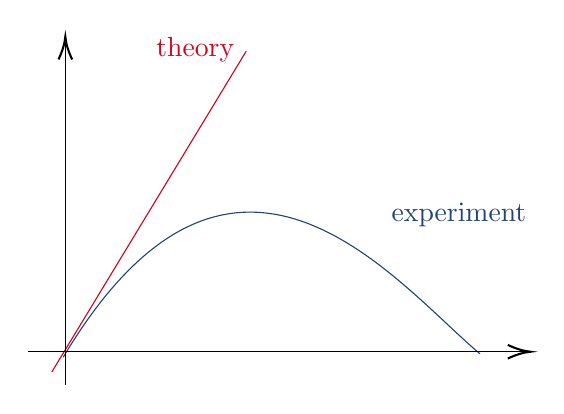
\begin{tikzpicture}[x=0.75pt,y=0.75pt,yscale=-1,xscale=1]
%uncomment if require: \path (0,300); %set diagram left start at 0, and has height of 300

%Straight Lines [id:da44773090746859867] 
\draw [color={rgb, 255:red, 208; green, 2; blue, 27 }  ,draw opacity=1 ]   (100.87,233.5) -- (194.5,79) ;
%Curve Lines [id:da7265875796819894] 
\draw [color={rgb, 255:red, 34; green, 68; blue, 114 }  ,draw opacity=1 ]   (106.37,226.38) .. controls (188.5,89) and (266.53,190.65) .. (307.14,224.76) ;
%Straight Lines [id:da8045363903004159] 
\draw    (89.5,223.76) -- (329.5,223.76) ;
\draw [shift={(331.5,223.76)}, rotate = 180] [color={rgb, 255:red, 0; green, 0; blue, 0 }  ][line width=0.75]    (10.93,-3.29) .. controls (6.95,-1.4) and (3.31,-0.3) .. (0,0) .. controls (3.31,0.3) and (6.95,1.4) .. (10.93,3.29)   ;
%Straight Lines [id:da5761614694400692] 
\draw    (107.37,240) -- (107.37,74) ;
\draw [shift={(107.37,72)}, rotate = 450] [color={rgb, 255:red, 0; green, 0; blue, 0 }  ][line width=0.75]    (10.93,-3.29) .. controls (6.95,-1.4) and (3.31,-0.3) .. (0,0) .. controls (3.31,0.3) and (6.95,1.4) .. (10.93,3.29)   ;

% Text Node
\draw (170,78) node  [color={rgb, 255:red, 208; green, 2; blue, 27 }  ,opacity=1 ] [align=left] {theory};
% Text Node
\draw (297,158) node  [color={rgb, 255:red, 34; green, 68; blue, 114 }  ,opacity=1 ] [align=left] {experiment};


\end{tikzpicture}
\end{figure}
\noindent This implies that the theory does not work for high energies. In order to have an unitary theory a requirement is 
\[\bar\sigma\leq\frac{4\pi}{s}\]
i.e. V-A theory preserves unitariety only if $\sqrt s\leq\sqrt{2\pi/G_F}\simeq 700$GeV. This implies that initial energies of particles in c.o.m. have to be smaller than $\approx 300$GeV.
\begin{figure}[H]
\centering


\tikzset{every picture/.style={line width=0.75pt}} %set default line width to 0.75pt        

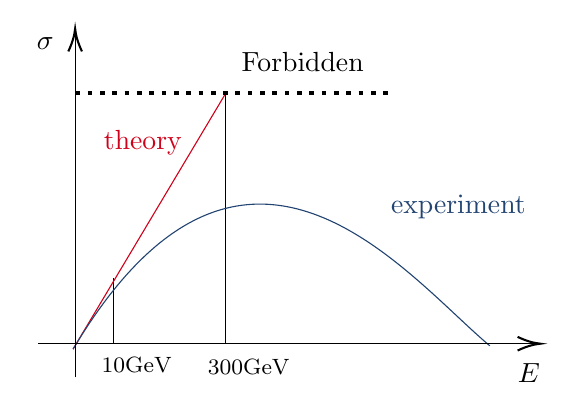
\begin{tikzpicture}[x=0.75pt,y=0.75pt,yscale=-1,xscale=1]
%uncomment if require: \path (0,300); %set diagram left start at 0, and has height of 300

%Straight Lines [id:da7811652857836433] 
\draw    (180,103) -- (180,224) ;
%Straight Lines [id:da7584225598218981] 
\draw    (126,192) -- (126,224) ;
%Straight Lines [id:da44773090746859867] 
\draw [color={rgb, 255:red, 208; green, 2; blue, 27 }  ,draw opacity=1 ]   (106.37,226.38) -- (180,103) ;
%Curve Lines [id:da7265875796819894] 
\draw [color={rgb, 255:red, 34; green, 68; blue, 114 }  ,draw opacity=1 ]   (106.37,226.38) .. controls (188.5,89) and (266.53,190.65) .. (307.14,224.76) ;
%Straight Lines [id:da8045363903004159] 
\draw    (89.5,223.76) -- (329.5,223.76) ;
\draw [shift={(331.5,223.76)}, rotate = 180] [color={rgb, 255:red, 0; green, 0; blue, 0 }  ][line width=0.75]    (10.93,-3.29) .. controls (6.95,-1.4) and (3.31,-0.3) .. (0,0) .. controls (3.31,0.3) and (6.95,1.4) .. (10.93,3.29)   ;
%Straight Lines [id:da5761614694400692] 
\draw    (107.37,240) -- (107.37,74) ;
\draw [shift={(107.37,72)}, rotate = 450] [color={rgb, 255:red, 0; green, 0; blue, 0 }  ][line width=0.75]    (10.93,-3.29) .. controls (6.95,-1.4) and (3.31,-0.3) .. (0,0) .. controls (3.31,0.3) and (6.95,1.4) .. (10.93,3.29)   ;
%Straight Lines [id:da1588459136106537] 
\draw [line width=1.5]  [dash pattern={on 1.69pt off 2.76pt}]  (107.5,103) -- (259.75,103) ;

% Text Node
\draw (140,127) node  [color={rgb, 255:red, 208; green, 2; blue, 27 }  ,opacity=1 ] [align=left] {theory};
% Text Node
\draw (292,158) node  [color={rgb, 255:red, 34; green, 68; blue, 114 }  ,opacity=1 ] [align=left] {experiment};
% Text Node
\draw (217,88) node   [align=left] {Forbidden};
% Text Node
\draw (326,238) node    {$E$};
% Text Node
\draw (93,79) node    {$\sigma $};
% Text Node
\draw (137,234) node  [font=\footnotesize] [align=left] {10GeV};
% Text Node
\draw (191,235) node  [font=\footnotesize] [align=left] {300GeV};


\end{tikzpicture}
\end{figure}

\subsubsection{Non renormalizabililty}

We saw that Fermi theory is not renormalizable, since $[G_F]=-2$ implies ultaviolet divergence at higher orders.
























\end{document}